In this chapter, we will discuss the experimental techniques that are used to fabricate twisted bilayer graphene devices. The fabrication of the devices is a very important step as many things in this step determine whether we will will observe certain feature in our measurements. In this experiment, we need to have a twist angle between the graphene to be close to magic angle, i.e., $1.1 ^o$. The thickness of the tunnel barrier hBN and the alignment of the flakes are also important in the making of these devices.

\section{Exfoliation of Graphene and hBN}

There are various ways of preparing graphene flakes. \cite{Bhuyan2016} The notable ones are Mechanical Exfoliation and Chemical Vapour Deposition (CVD). CVD can be used to grow large scale continuous graphene sheets in the order centimeters. But this method doesn't produce graphene flakes that have good electron mobility like in the case of Mechanical Exfoliation. We use Mechanical Exfoliation in our experiments.

In this method, we exfoliate graphene flakes onto Si-SiO2 substrate. We have Si-SiO2 substrate cut into small pieces of approximately 1.5cm*1.5cm. We then clean the wafers using sonication, in which the wafers are put in a beaker of acetone and sonicated in either normal or soft mode for 5mins. The wafers are thin dipped in IPA and blow dryed using N2. These steps remove the organic adsorbates from the substrate surface. We worked with three variations of Mechanical Exfoliation:

\begin{itemize}
    \item Conventional Exfoliation:
    We place a chunk of natural graphite on a Scotch tape and subsequently cleave it to the fresh regions of the tape, uniformly distributing on the tape. This tape is called the Master Tape. The graphite crystals are then transferred from Master Tape onto a new tape by adhering the second tape to the first and slowly peeling it away. This process is repeated till thin translucent graphite crystals containing tape is made. This step ensures that we have flat regions of graphite on the tape surface. This tape is then stuck on the substrate and we gently apply pressure using a plastic dropper. We peel off the tape slowly. When the tape is removed, van der Waals force between tthe substrate and the top layers of the graphite crystals will pull down flakes of graphite ranging from 0.34nm (monolayer graphene) to hundreds of nanometers
    \item Hot Exfoliation:
    We follow the same steps as in conventional exfoliation, with one variation. We heat the substrate using a hot plate at $100 ^o C$ for 2-3 mins before sticking the tape onto it. This will improve the adhesion between graphite crystals and substrate.
    \item Oxygen Plasma Exfoliation:
    Here also we follow the same steps as in conventional exfoliation, with one variation. We clean the substrate using oxygen plasma cleaner before sticking the tape on it. This step helps in removing adsorbates from the surface of the substrate, hence improving the flake transfer, both in number and size.
   
    \end{itemize}

We use Hot Exfoliation to get graphene flakes for our devices. The reason we don't use oxygen plasma is because the flakes obtained by this method are hard to pickup using dry transfer method (sec 3.3). We are looking for large monolayer graphene.

We use conventional Mechanical Exfoliation to get hexagonal Boron Nitride (hBN) flakes. The method is similar to that for graphene, with hBN crystals used instead of graphite while making the master tape. We use hBN crystals from Japan, that are known to give good quality thin flakes. We are looking for hBN with two different thicknesses - <5nm (thin hBN) and around 30nm (thick hBN). The thin hBN is used as the tunneling barrier between twBLG and gold pads, while thick hBN is used as top and bottom hBN next to the gate.

\section{Flake selection}
\section{Stamp creation}

Stacks of graphene and hBN are created by putting them on top of each other, using Pickup and Transfer process. This process involves the use of polymer stamps that can stick to a flake and pick it up. The stamp consists of a coverslip with PPC or PC on hemispherical PDMS. The first step is to make the PDMS coverslips. The protocol is as follows:
\begin{enumerate}
\item Sonicate coverslips in acetone, wash with IPA and blowdry in N2.
\item Bake the coverslips for 5 minutes at 150 $^{\circ}$ C to remove moisture.
\item Mix 10 parts PDMS with 1 part curing agent on a clean glass slide using a clean toothpick.
\item Put PDMS onto the coverslips by using a toothpick, picking up some PDMS mixture by holding the toothpick vertically.
\item Bake the coverslips at 150 $^{\circ}$ C for 30 min.
\end{enumerate}
A layer of PPC or PC is now added on PDMS that is used to pickup the flakes. The steps for this are:
\begin{enumerate}
\item Put a drop or two of PPC (15 percent PPC in anisole) or PC (6 percent PC in Chloroform) on PDMS coverslip using a dropper.
\item Spin coat it at 3000rpm for 30s, by attaching the coverslip to the spin coater with a double sided tape.
\item Keep the coverslip immediately on the hot plate to bake at $70 ^o C$ for 10 mins.
\end{enumerate}
PPC or PC solution has to be kept ready before starting stamp making. For making PPC solution: 
\begin{enumerate}
\item Take a small glass bottle, wash it and heat it at $80 ^o C$ for 1hr 30min. \item Measure and transfer 10ml of Anisole in the bottle and add 1.5g of PPC crystals in it, making a solution.
\item Shake the bottle vigorously and leave overnight.
\end{enumerate}
For making PC solution:
\begin{enumerate}
\item Wash a small glass bottle. 
\item Measure and transfer 3ml of Chloroform in the bottle and add 0.18g of PC crystals in it.
\item Leave the bottle overnight.
\end{enumerate}
This coverslip is stick on the transfer stage using a metal stick. This is done with following steps:
\begin{enumerate}
\item Keep the coverslip on the metal stick and add EL-9 along the edges of the coverslip using a micro pipette.
\item Bake this at 90 $^{\circ}$ C on the hot plate for 2-3 mins.
\item Attach the metal stick to the stage using double sided tape.
\end{enumerate}

\section{Pickup and Transfer Process}

Let's discuss the pickup and transfer process. After the PPC-PDMS and/or PC-PDMS stamp is ready, this process called the dry transfer technique \cite{Kim16} \cite{Wang614} is started in the transfer setup (shown in fig.). PC-PDMS stamp is used for thin hBN transfer and PC-PDMS stamp for everything else. The choice is based on the optimisation. The pickup and transfer protocol is as follows:

Part 1: Making a transfer boundary
\begin{enumerate}
\item Cover the microscope stage with Kaptan tape and put a little square of double sided tape on top of it.
\item Now a transfer boundary is made on PDMS. A piece of clean silicon wafer is stuck on the double sided tape and transfer stage metal stick is moved between the microscope stage and the objective.
\item Using the Piezo the coverslip is moved vertically till the PPC-PDMS or PC-PDMS is in focus and center the region with PDMS. 
\item The PDMS is moved up and the empty wafer is brought into focus, and the stage heater temperature is set to $63 ^o C$ for PPC ($130 ^o C$ for PC).
\item The transfer stage is moved down slowly using the Piezo motors while keeping the wafer in focus. When the PDMS touches the wafer, a circle forms on the coverslip. The coverslip is held there for 5 seconds and then moved up.  A circular boundary will be seen on the PDMS after this step. This is the transfer boundary where the PDMS will pick up flakes.
\item Finally, remove the wafer and the Kaptan tape.
\end{enumerate}
Part 1 can be skipped once we are comfortable with the whole process.

Part 2: Pickup Step
\begin{enumerate}
\item Mount the wafer with the hBN/graphene flake to be picked in the same way as before, on the double double sided tape.
\item Follow similar steps as before, except now center the flake to be picked, directly under the transfer circle of PDMS.
\item Once the PDMS touches the wafer, go down till the circle spreads over the flake that needs to be picked.
\item Wait for 10 mins and turn off the heating.
\item Wait till the temperature comes down to around $35 ^o C$. Next, move the PDMS up and confirm if the flake got picked.
\item Finally, remove the wafer and the Kaptan tape.
\end{enumerate}

Part 3: Transfer Step

Now there are two things that can be done. Either we keep on picking up flakes or transfer the flake/stack onto a clean wafer/gold pad. For the first case, we continue with the steps as above. We will have to take care of alignment during these steps. For the transfer, we perform the following steps:
\begin{enumerate}
\item Cover the microscope stage with Kaptan tape and put a little square of double sided tape on top of it.
\item Mount the wafer onto which the flake has to be transferred on the double sided tape and heat the stage to $75 ^o C$ for PPC ($180 ^oC$ for PC)
\item Touch the PDMS with the flake over the area to be transferred on and wait for 10 min.
\item Move the PDMS up and check if the flake got transferred.
\item Remove the wafer and the Kaptan tape.
\item Remove the coverslip from the transfer stick by dissolving EL-9 using acetone.
\item Finally, clean the coverslip and the wafer. They are kept in Anisole overnight (Chloroform for 2 hours) to dissolve the PPC (PC). Wash them with IPA (IPA and acetone), and blowdry with $N_2$.
\end{enumerate}
\begin{figure}[H]
     \centering
     \begin{subfigure}[b]{0.4\textwidth}
         \centering
         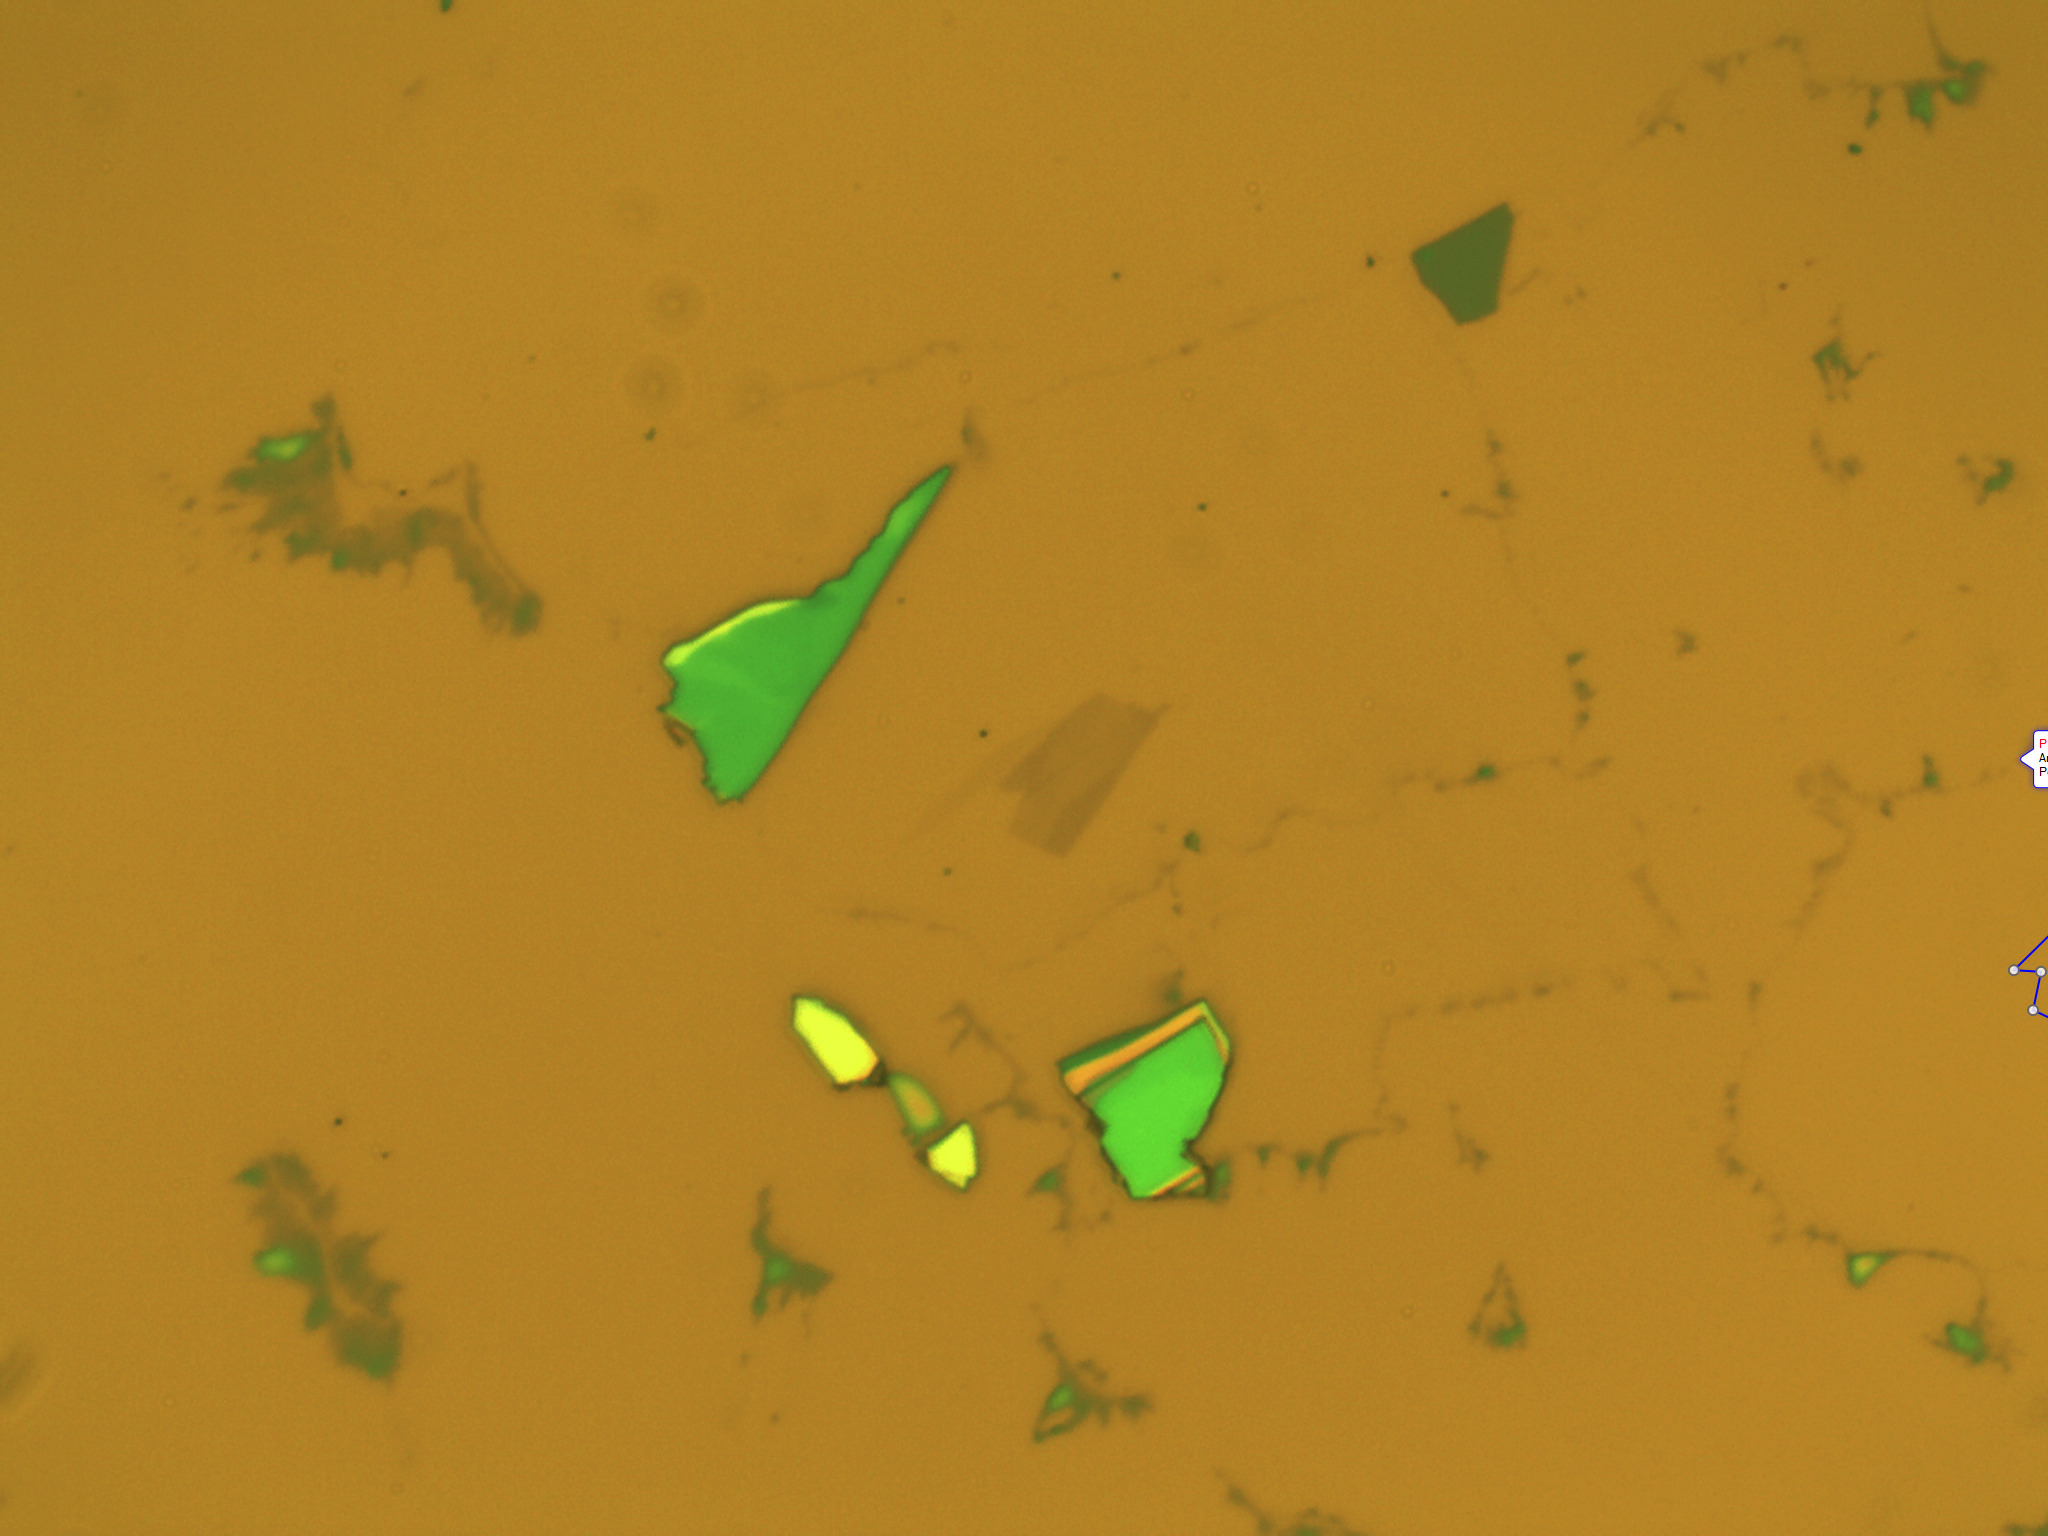
\includegraphics[width=\textwidth]{figures/hbn_before_pickup.jpg}
         \caption{hBN before pickup}
     \end{subfigure}
    \qquad
     \begin{subfigure}[b]{0.4\textwidth}
         \centering
         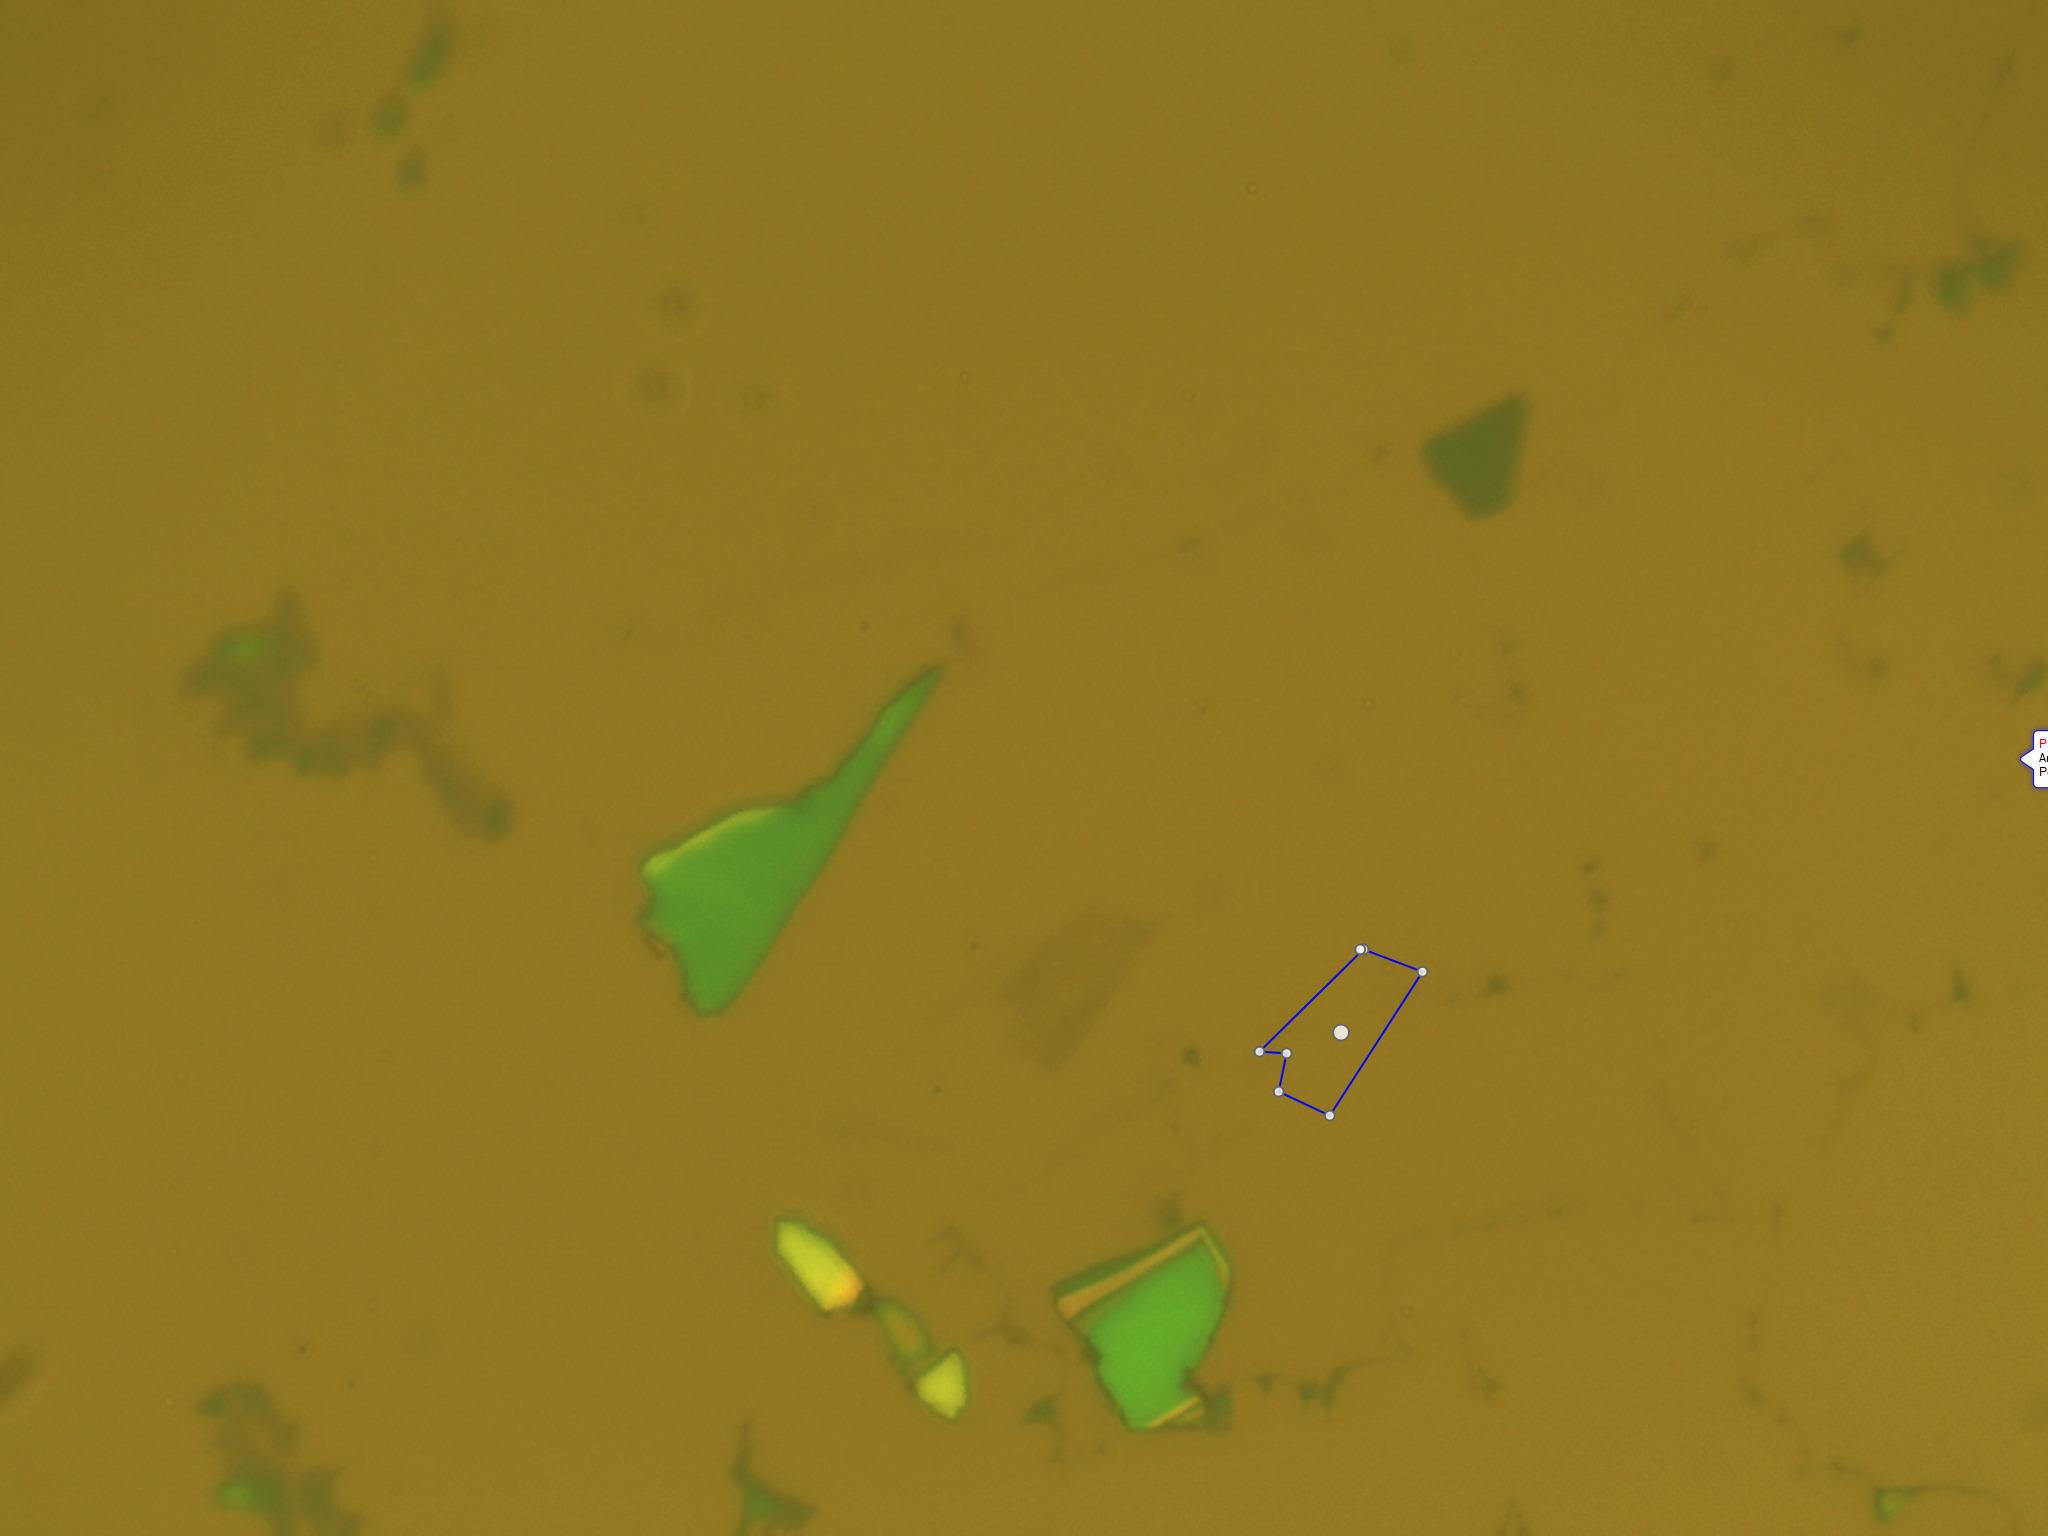
\includegraphics[width=\textwidth]{figures/hbn_through_pc.jpg}
         \caption{hBN through PC}
     \end{subfigure}
    \begin{subfigure}[b]{0.4\textwidth}
         \centering
         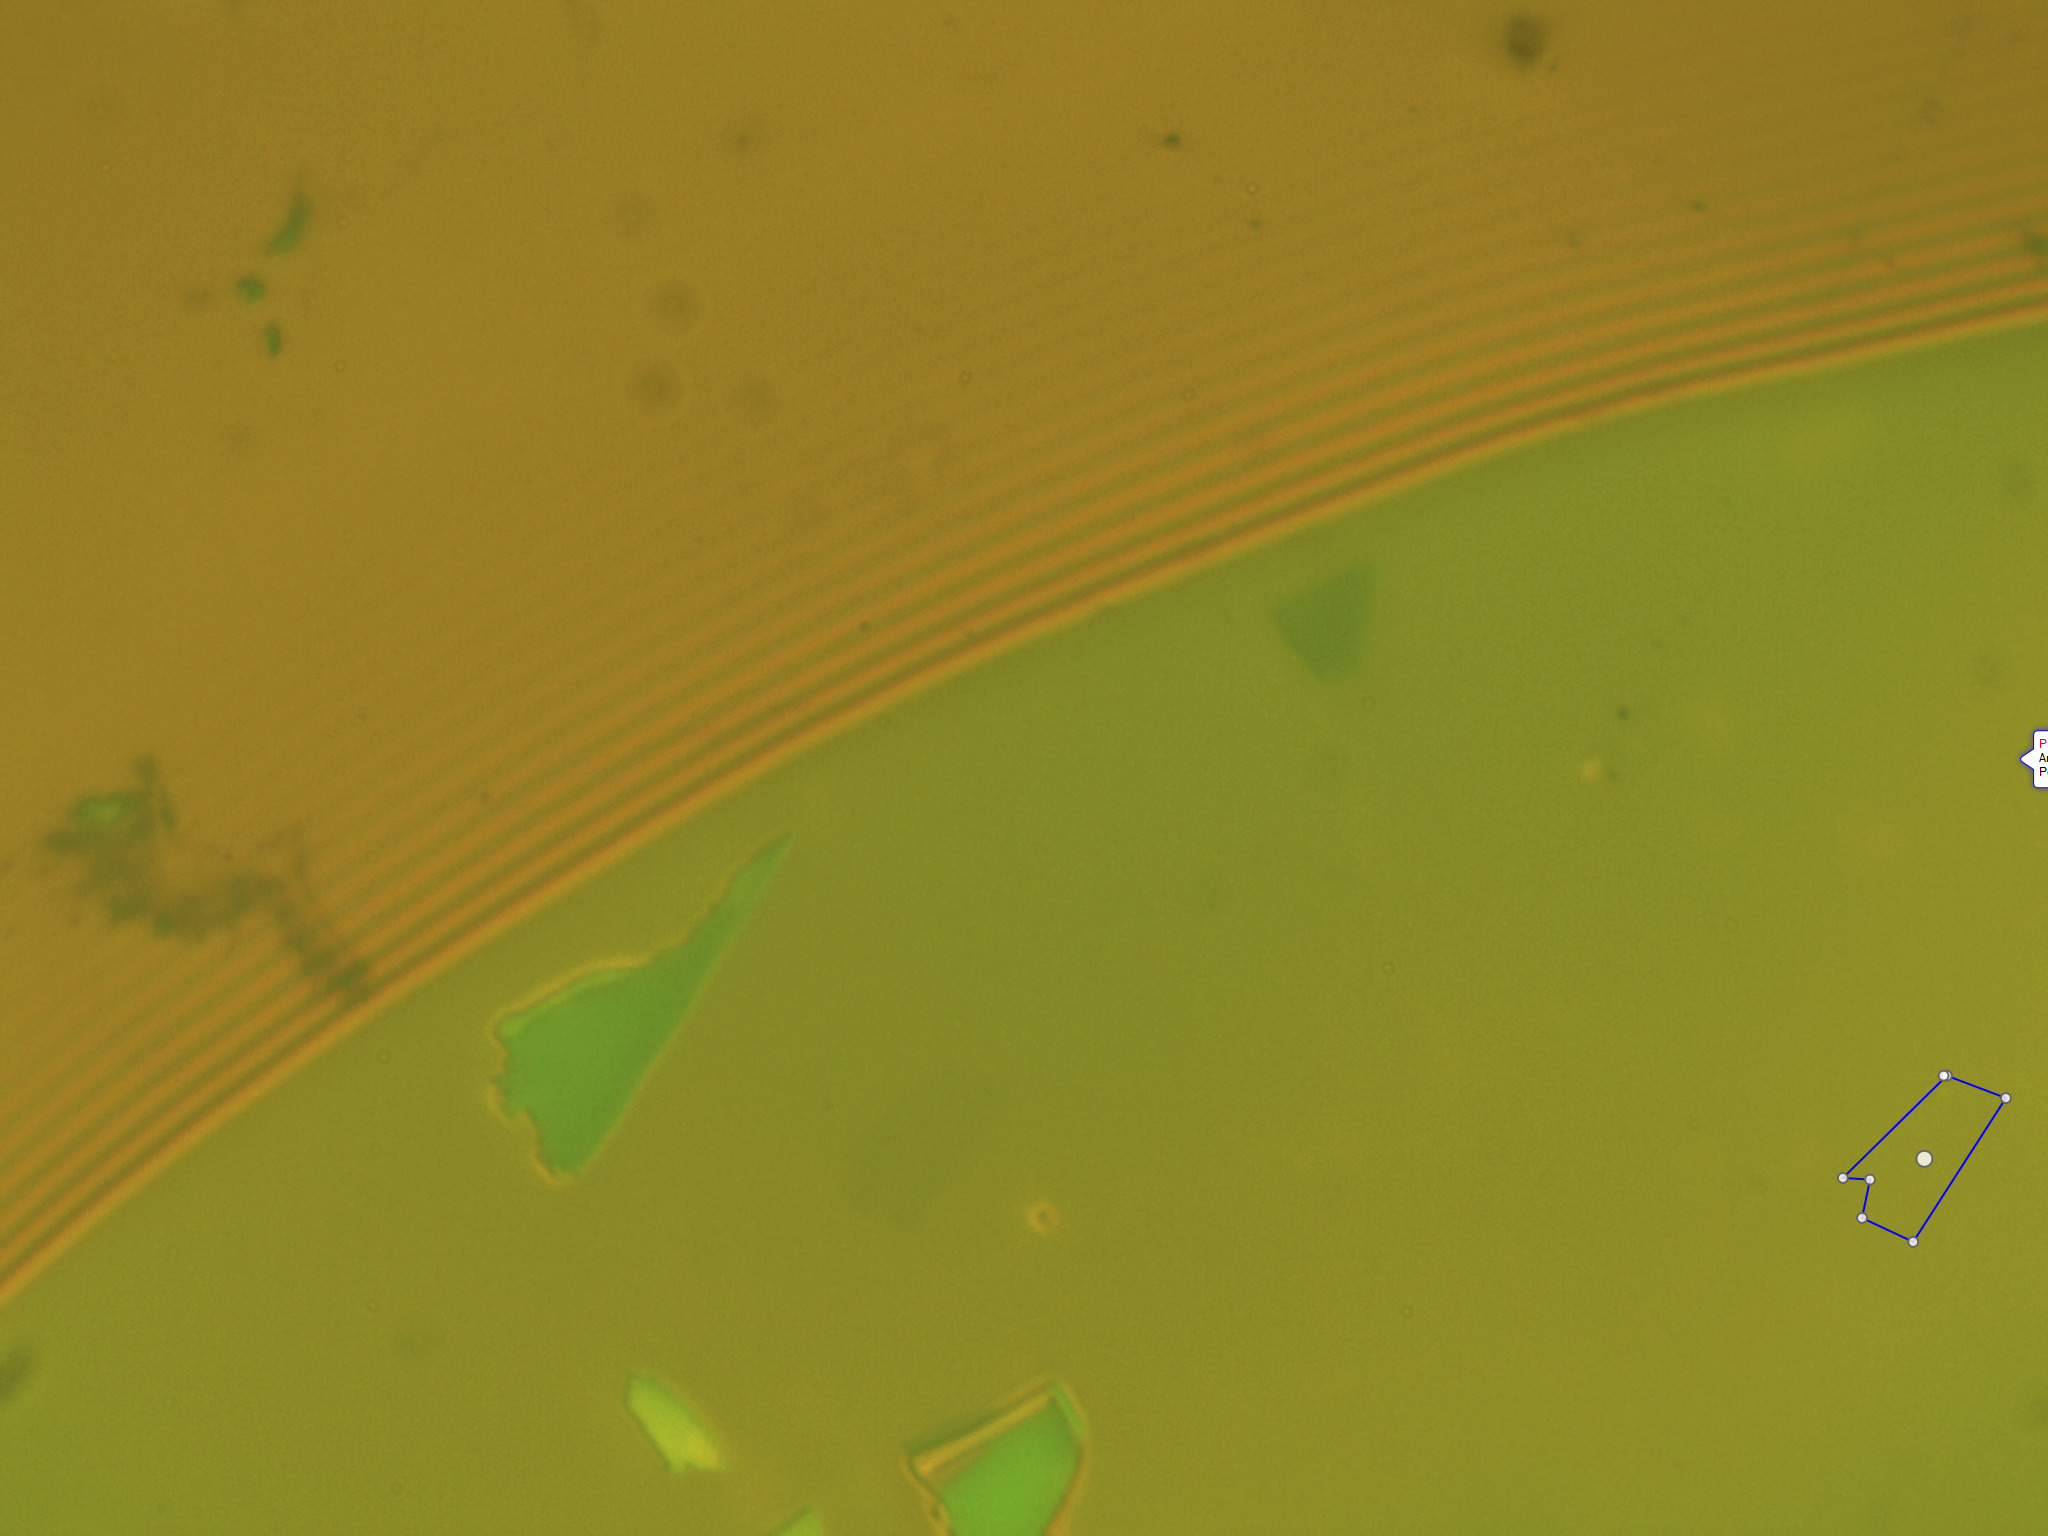
\includegraphics[width=\textwidth]{figures/during_pickup.jpg}
         \caption{During Pickup}
     \end{subfigure}
     \qquad
     \begin{subfigure}[b]{0.4\textwidth}
         \centering
         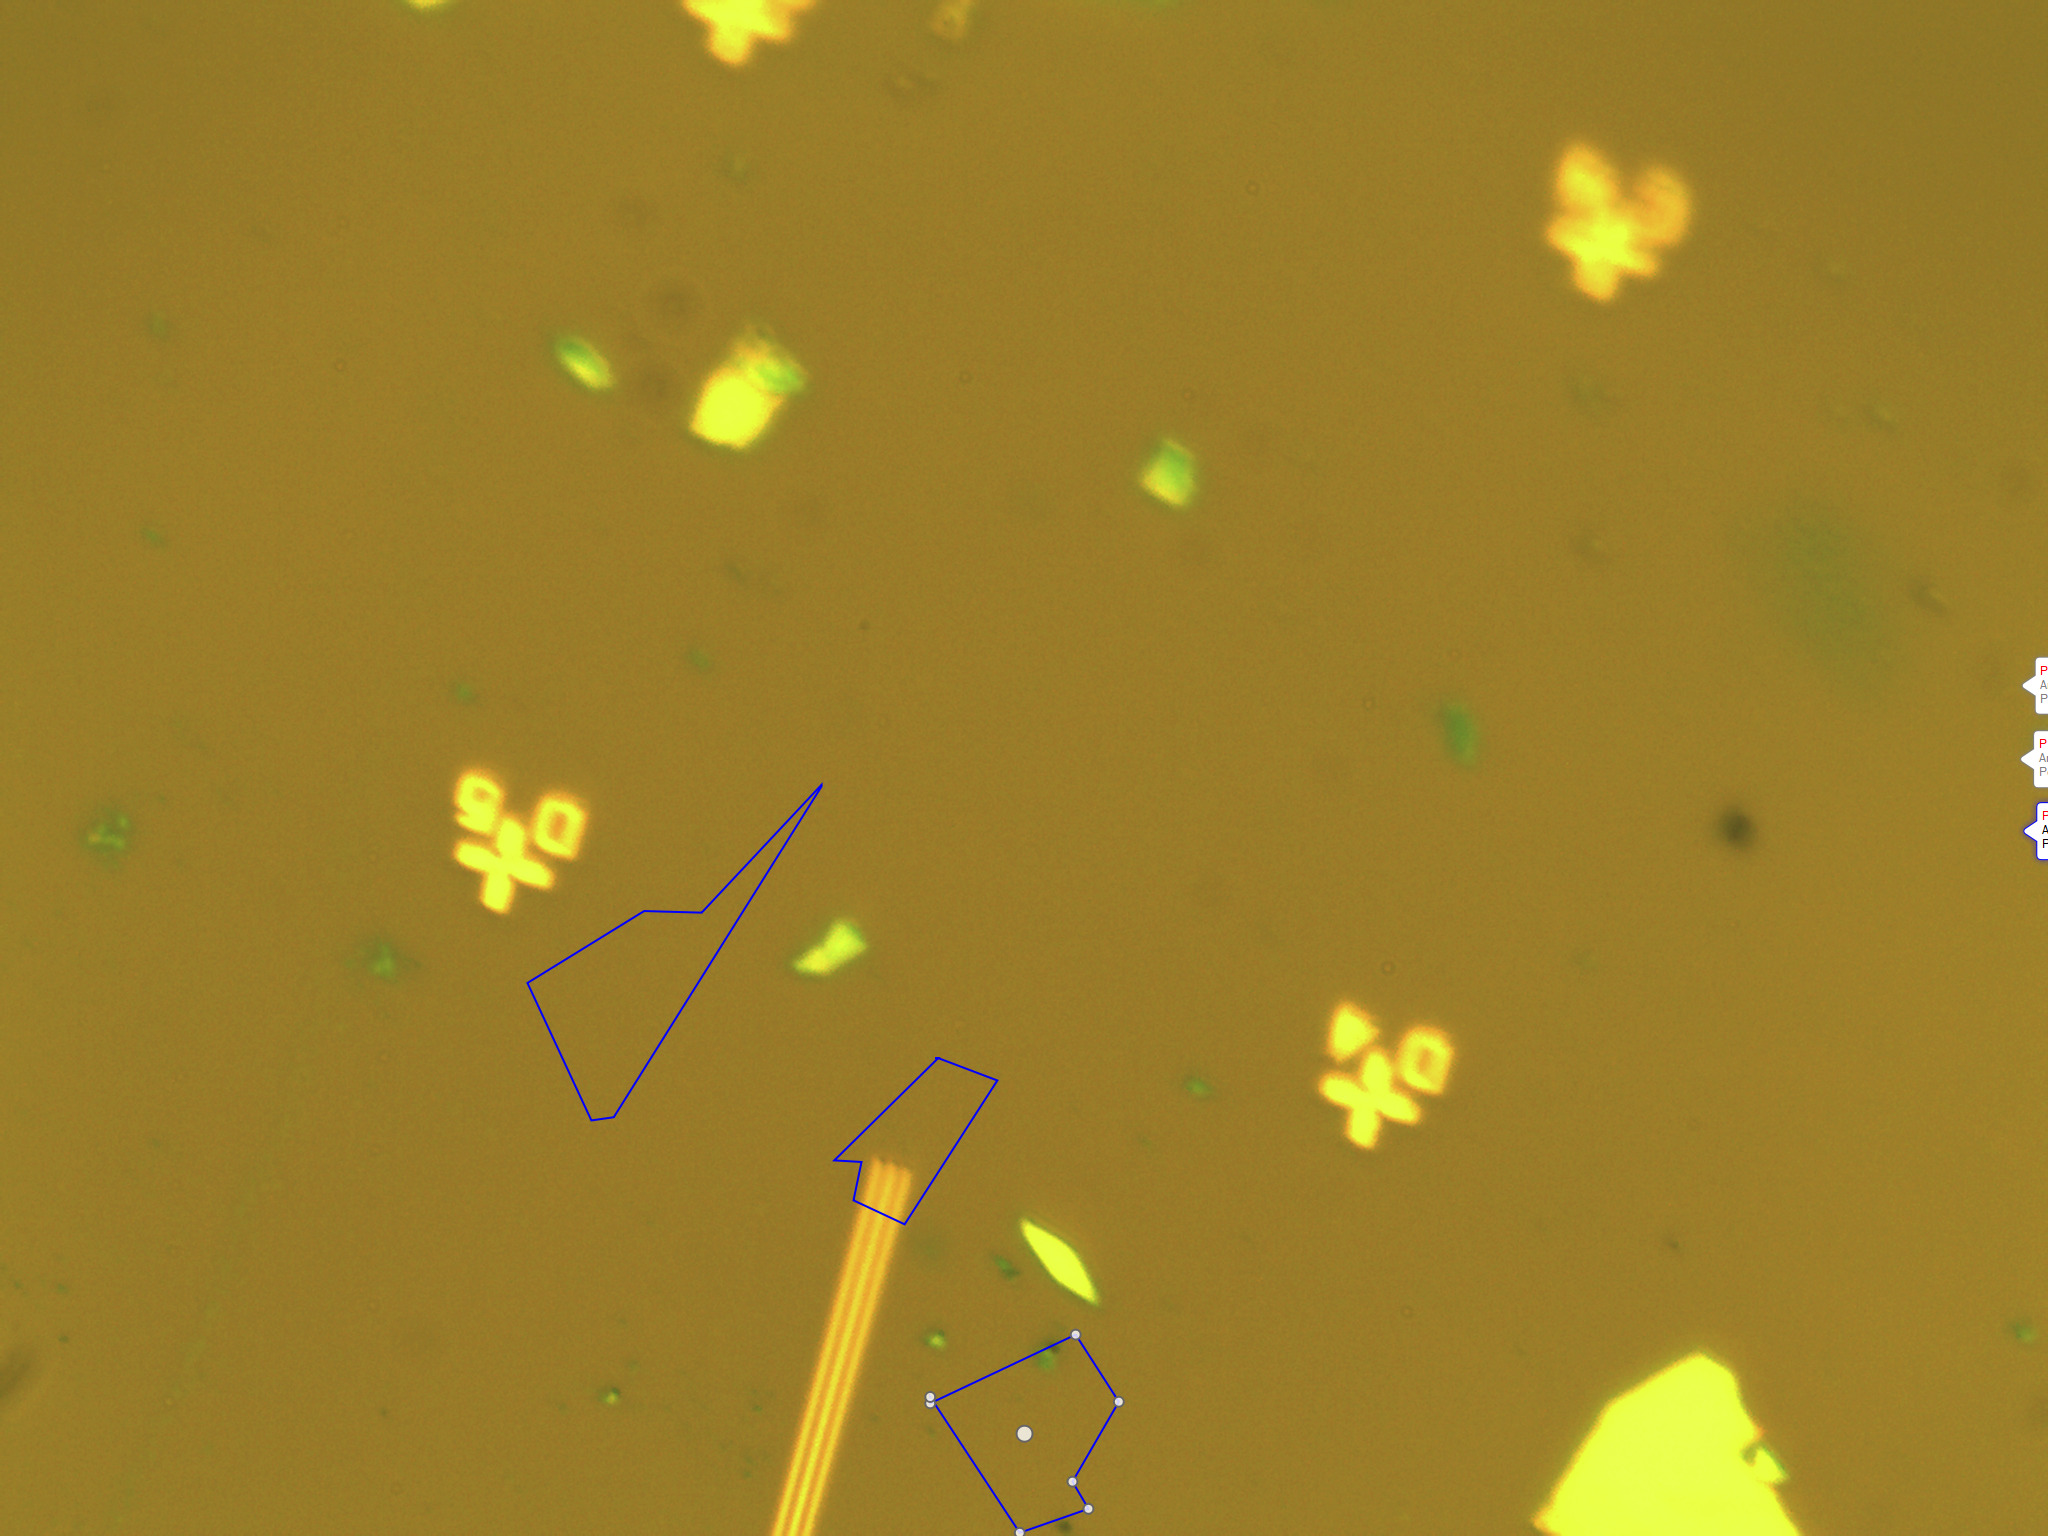
\includegraphics[width=\textwidth]{figures/gold_pad.jpg}
         \caption{Gold pad}
     \end{subfigure}
     \begin{subfigure}[b]{0.4\textwidth}
         \centering
         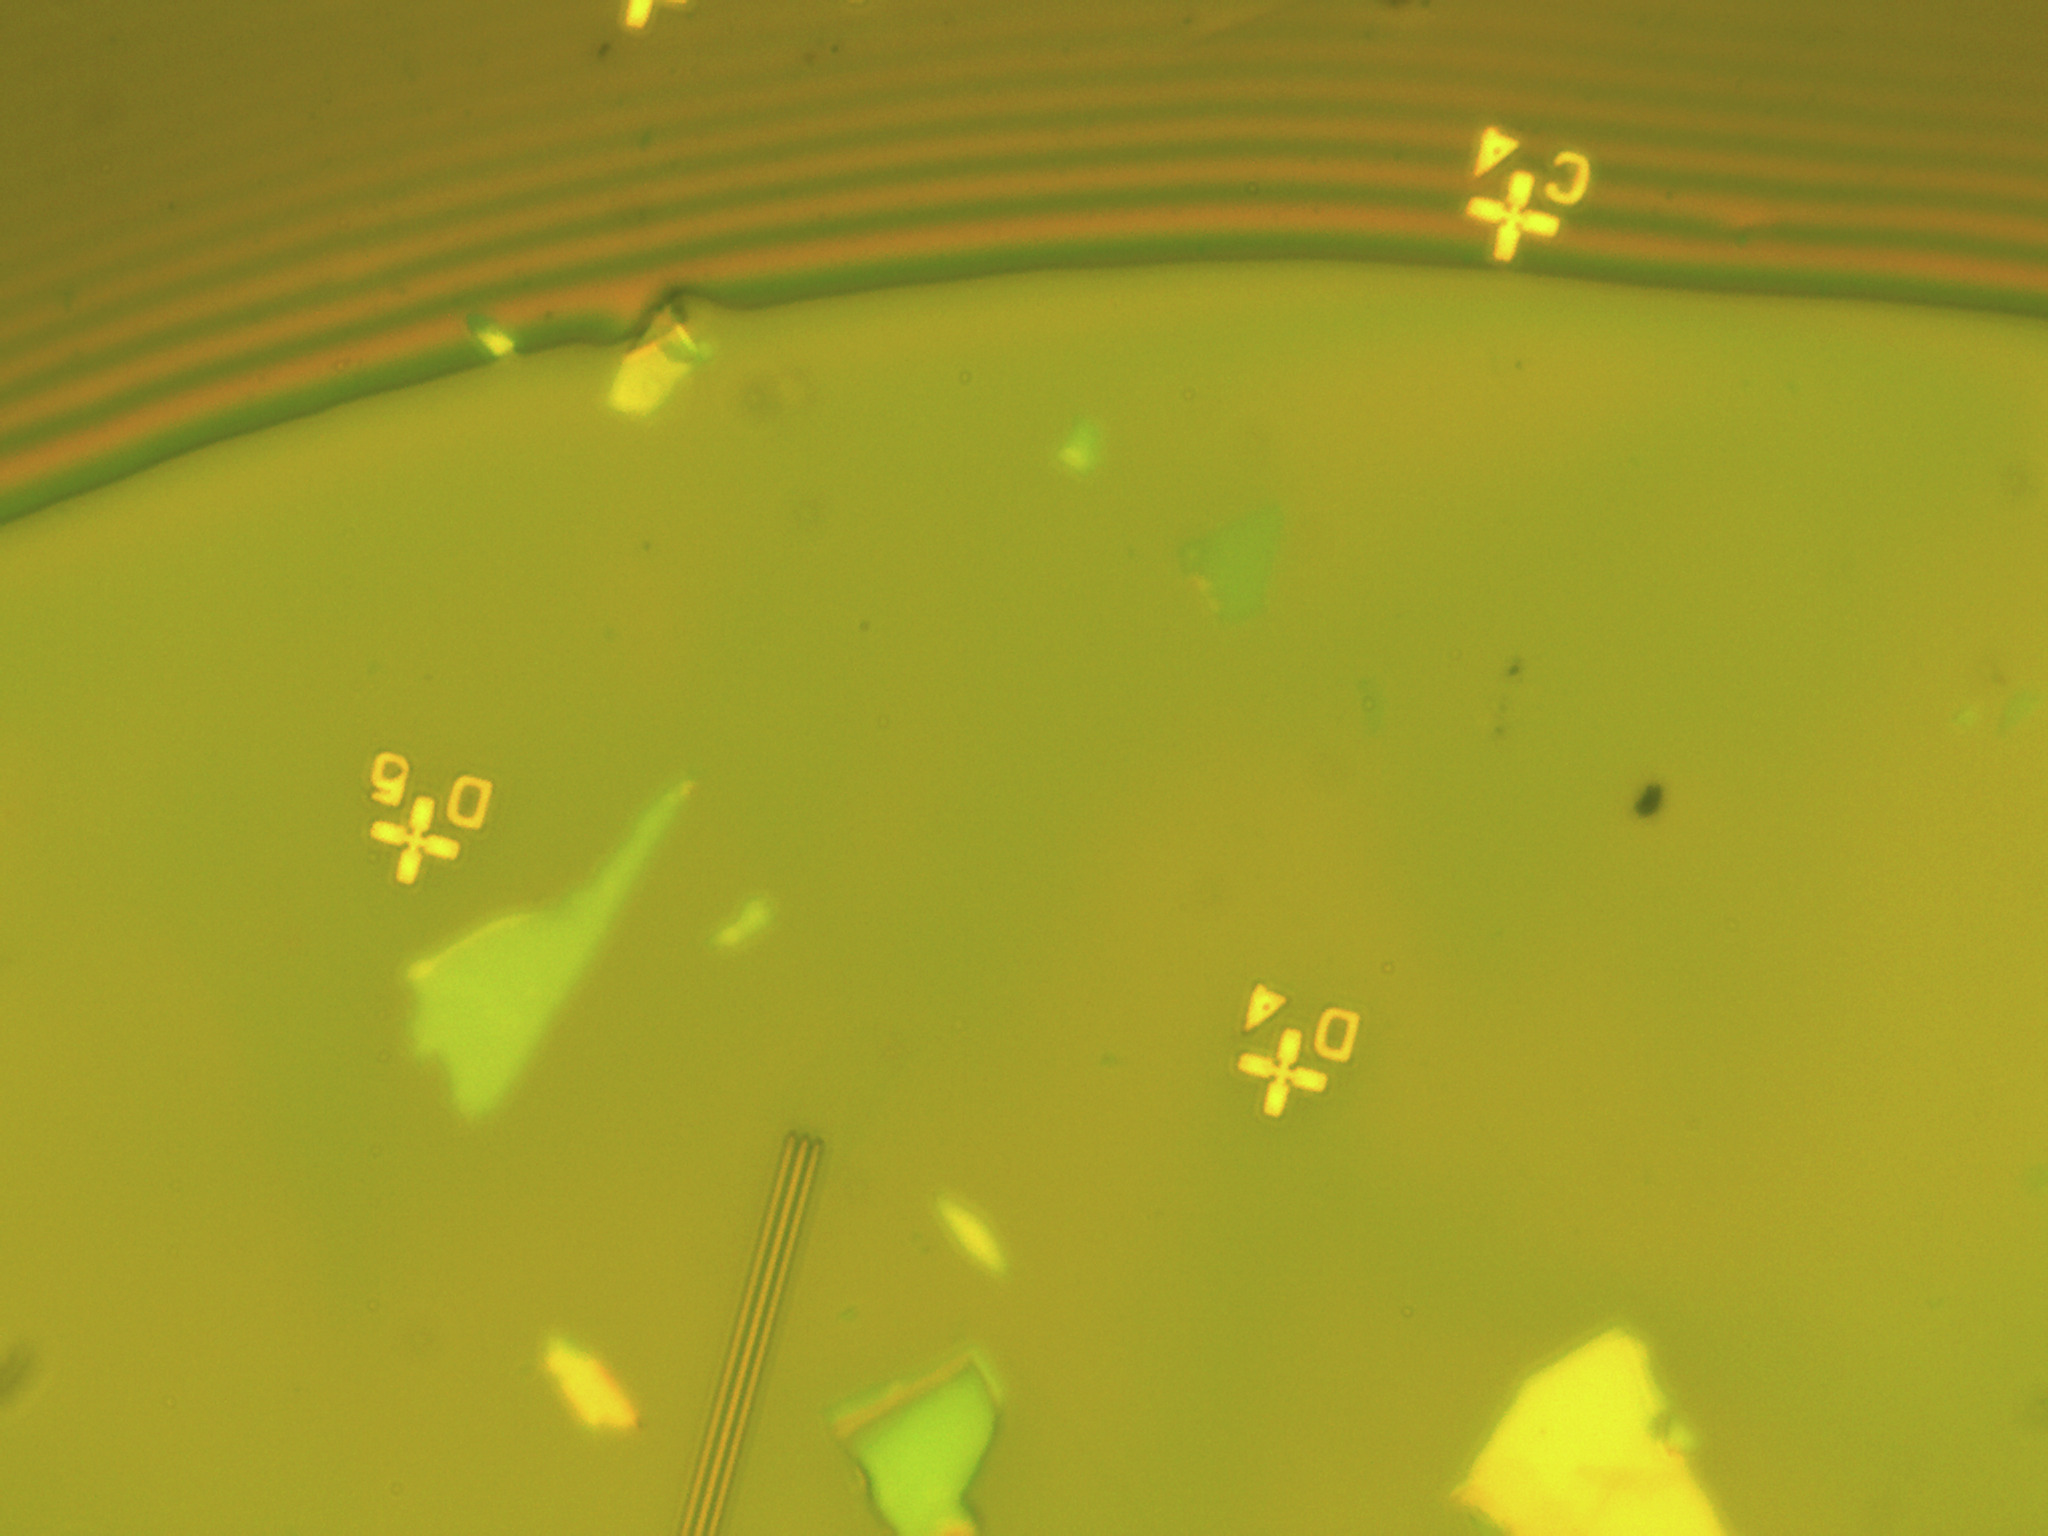
\includegraphics[width=\textwidth]{figures/during_transfer.jpg}
         \caption{During Transfer}
     \end{subfigure}
     \qquad
     \begin{subfigure}[b]{0.4\textwidth}
         \centering
         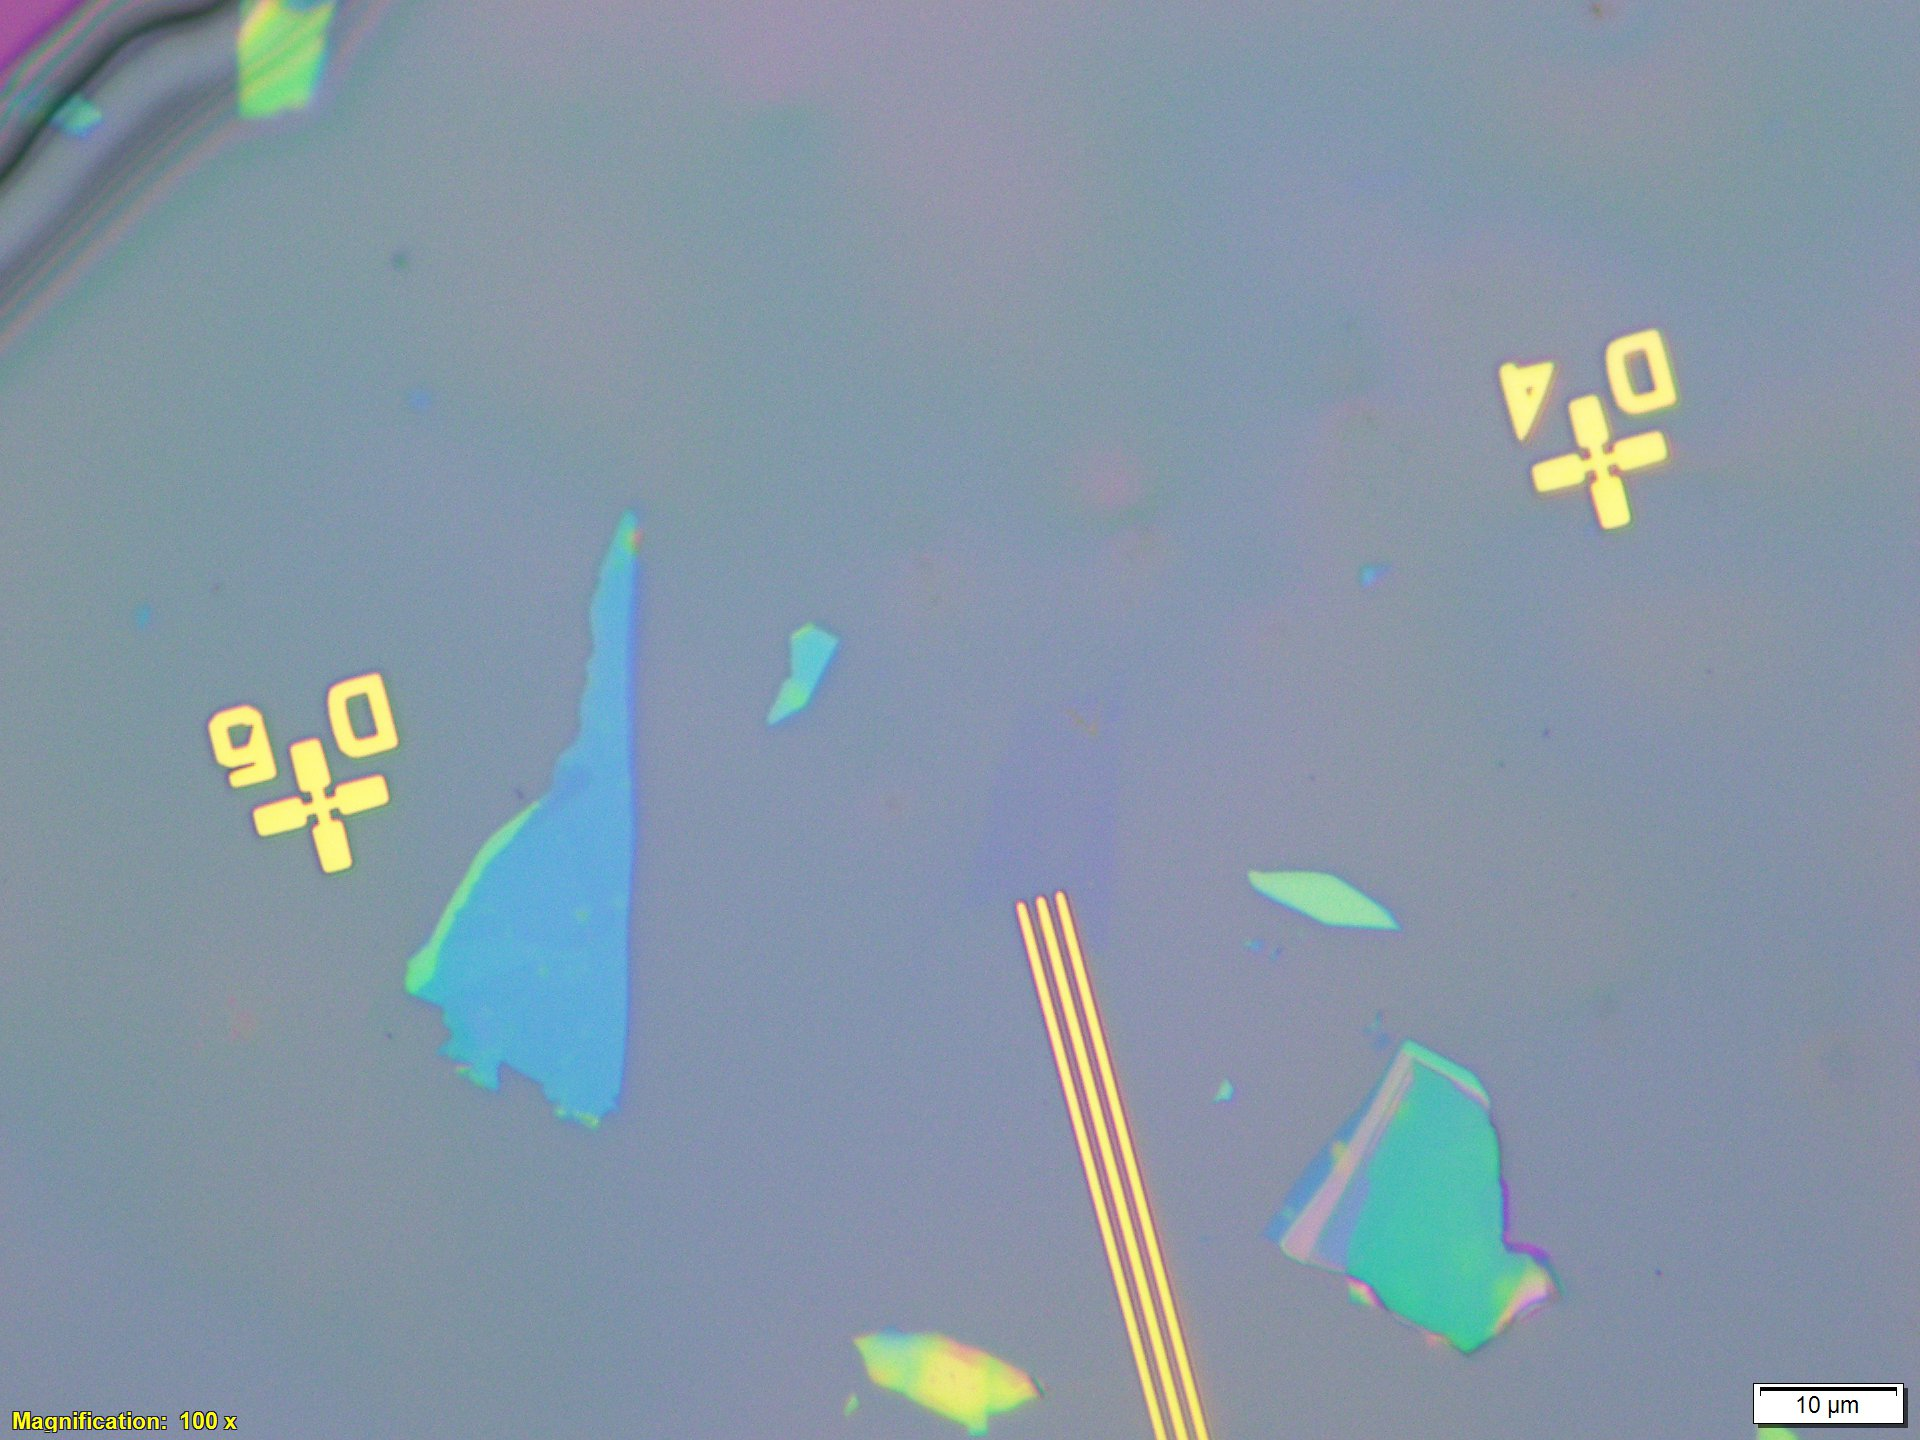
\includegraphics[width=\textwidth]{figures/after_transfer.jpg}
         \caption{After Transfer}
     \end{subfigure}
        \label{fig:hbnongoldpad}
    \caption{Pickup and Transfer of thin hBN on gold pad}
\end{figure}

\section{Twisted Bilayer Graphene Fabrication}

We need to make hBN-graphene-graphene-hBN-gold pad stacks for our devices. Here the top hBN encapsulates the twisted bilayer graphene. The two graphene flaskes are aligned at magic angle of $1.1 ^o$. The hBN on the gold pad acts as a tunneling barrier. We have two parts in the whole process. One is to transfer thin hBN onto gold pad, the other is to make hBN-graphene-graphene stack on PPC. We follow the protocols as mentioned in sec 3.3, with one extra step during the stack preparation. We cut the graphene using a tip and pickup one half of the flake with hBN, twist the stage at magic angle of $1.1 ^o$ and pickup the other of the flake with graphene. We anneal the hBN-gold pad substrate, which helps in removing residues present on the flake, making it better for using it in our device. We then transfer the hBN-graphene-graphene stack onto the hBN-gold pad substrate, giving us the final stack. We can then proceed with drawing contacts. 